\documentclass[12pt,aspectratio=169]{beamer}
\usepackage[T1]{fontenc}
\usepackage{lmodern}
\usepackage{amsmath,amssymb,array,booktabs,tabularx,tikz}
% Add language support appropriate to the source, if needed.
% Keep this preamble inline in every delivered deck.
\definecolor{GEInk}{HTML}{132A3E}
\definecolor{GETeal}{HTML}{17675E}
\definecolor{GEFooter}{HTML}{EAF2F1}
\setbeamercolor{background canvas}{bg=white}
\setbeamercolor{normal text}{fg=GEInk,bg=white}
\setbeamercolor{structure}{fg=GETeal}
\setbeamercolor{frametitle}{fg=GEInk}
\setbeamercolor{GE footer}{fg=GETeal,bg=GEFooter}
\setbeamerfont{normal text}{family=\sffamily,size=\normalsize}
\setbeamerfont{title}{size=\huge,series=\bfseries}
\setbeamerfont{subtitle}{size=\normalsize,series=\bfseries}
\setbeamerfont{frametitle}{size=\Large,series=\bfseries}
\setbeamerfont{framesubtitle}{size=\normalsize,series=\mdseries}
\setbeamerfont{GE footer}{size=\footnotesize}
\setbeamersize{text margin left=9mm,text margin right=9mm}
\setbeamertemplate{navigation symbols}{}
\setbeamertemplate{headline}{}
\setbeamercovered{invisible}
\setbeamertemplate{frametitle}{%
  \vskip.5em
  {\usebeamerfont{frametitle}\strut\insertframetitle\strut\par}%
  \ifx\insertframesubtitle\empty\else
    {\usebeamerfont{framesubtitle}\strut\insertframesubtitle\strut\par}%
  \fi
  \vskip.25em
}
\setbeamertemplate{footline}{%
  \begin{beamercolorbox}[wd=\paperwidth,ht=3ex,dp=1.3ex,
    leftskip=9mm,rightskip=9mm]{GE footer}%
    \usebeamerfont{GE footer}\insertsectionhead\hfill
    \insertframenumber/\inserttotalframenumber
  \end{beamercolorbox}%
}
\setlength{\parindent}{0pt}
\setlength{\parskip}{.35em}
\setlength{\tabcolsep}{4pt}
\renewcommand{\arraystretch}{1.22}
\AtBeginEnvironment{frame}{\raggedright}
\addtobeamertemplate{frametitle}{}{%
  \setlength{\abovedisplayskip}{6pt plus 2pt minus 2pt}%
  \setlength{\belowdisplayskip}{6pt plus 2pt minus 2pt}%
  \setlength{\abovedisplayshortskip}{6pt plus 2pt minus 2pt}%
  \setlength{\belowdisplayshortskip}{6pt plus 2pt minus 2pt}%
}

\usepackage{pgfplots}
\pgfplotsset{compat=1.18}
\newif\ifGTenHighlights
\GTenHighlightstrue
% \GTenHighlightsfalse % Uncomment to disable instructional highlights.
\tikzset{ge marker/.style={rectangle,rounded corners=1mm,draw=none,
  fill=#1,fill opacity=.32,text opacity=1,text=GEInk,
  inner xsep=.6mm,inner ysep=.3mm,outer sep=0pt}}
\makeatletter
\newcommand{\GEHighlightMath}[2]{%
  \tikz[baseline=(gehl.base)]\node[ge marker=\GECurrentRole]
    (gehl) {$\m@th#1#2$};}
\newcommand{\GEHighlight}[2]{%
  \ifGTenHighlights\begingroup\def\GECurrentRole{#1}%
  \ifmmode\mathpalette\GEHighlightMath{#2}%
  \else\tikz[baseline=(gehl.base)]\node[ge marker=#1](gehl){#2};\fi
  \endgroup\else#2\fi}
\makeatother
% Keep rows, rules, and table structure outside this space-reserving command.
\newcommand{\GERevealCell}[2]{\leavevmode\leavevmode\visible<#1->{#2}}



\usetikzlibrary{calc}
\definecolor{Mass}{HTML}{86BFF0}
\definecolor{Cumulative}{HTML}{43A5C9}
\definecolor{Quantity}{HTML}{FFBB55}
\definecolor{Outcome}{HTML}{BC9DE0}
\colorlet{cTwoMassColor}{blue!75!black}
\colorlet{cTwoCDFColor}{cyan!65!blue!80!black}
\colorlet{cTwoGuideColor}{cTwoMassColor!35}
\ifGTenHighlights\else
\colorlet{cTwoMassColor}{black}\colorlet{cTwoCDFColor}{black}\colorlet{cTwoGuideColor}{gray}
\fi
% Base graph palette stays fixed when temporary instructional highlights clear.
\newcommand<>{\H}[2]{\leavevmode\begingroup
  \alt#3{\def\GEOpacity{.32}}{\def\GEOpacity{0}}%
  \ifGTenHighlights\else\def\GEOpacity{0}\fi
  \tikzset{ge marker/.append style={fill opacity=\GEOpacity}}%
  \GEHighlight{#1}{#2}\endgroup}
\newcommand{\cTwoValue}[1]{\GEHighlight{Quantity}{#1}}
\newcommand{\cTwoOutcome}[1]{\GEHighlight{Outcome}{#1}}
\newcommand{\cTwoMassHL}[1]{\GEHighlight{Mass}{#1}}
\newcommand{\cTwoCDFHL}[1]{\GEHighlight{Cumulative}{#1}}
\newcommand{\Blank}[1]{\rule{0pt}{.56cm}#1}
% Fixed-size drawing area. x = 1 cm / USD; y = 3.1 cm / probability unit.
\newcommand{\TickLabel}[1]{#1}
\newcommand{\PMFTickLabel}[1]{\ifnum#1=0\H<3>{Quantity}{#1}\else\ifnum#1=2\H<4>{Quantity}{#1}\else\H<5>{Quantity}{#1}\fi\fi}
\newcommand{\GraphStart}[1]{\begin{tikzpicture}[x=1cm,y=3.1cm]
\path[use as bounding box] (-1.85,-.28) rectangle (5.65,1.24);\begin{pgfinterruptboundingbox}
\foreach \y in {0,.25,.5,.75,1}{\draw[gray!15] (-1,\y)--(5.3,\y);
\node[anchor=east,font=\small] at (-1.1,\y) {\pgfmathprintnumber{\y}};}
\draw[->] (-1,0)--(5.5,0); \draw[->] (-1,0)--(-1,1.12);
\foreach \x in {0,2,4}{\draw (\x,0)--(\x,-.025);\node[below,font=\small] at (\x,-.025){\TickLabel{\x}};}
\node[anchor=south west,font=\small] at (-1,1.13){#1};
\node[font=\small] at (2,-.22){$x$ (USD)};}
\newcommand{\GraphEnd}{\end{pgfinterruptboundingbox}\end{tikzpicture}}
\newcommand{\Step}[4]{\draw[cTwoCDFColor,thick,#4] (#1,#3)--(#2,#3);}
\newcommand{\Open}[2]{\draw[cTwoCDFColor,fill=white,thick] (#1,#2) circle[radius=2pt];}
\newcommand{\Closed}[2]{\fill[cTwoCDFColor] (#1,#2) circle[radius=2pt];}
\newcommand{\FullCDF}{\Step{-1}{0}{0}{<-}\Step{0}{2}{.15}{}\Step{2}{4}{.75}{}\Step{4}{5.3}{1}{->}
\Open{0}{0}\Open{2}{.15}\Open{4}{.75}\Closed{0}{.15}\Closed{2}{.75}\Closed{4}{1}}
\title{Constructing PMF and CDF Tables and Graphs}
\subtitle{Grade 10 · Term 2 · Lesson 1 · 2026--2027}
\author{}\date{}
\newcommand{\GEOfficialCriterion}{\textbf{C2:} Interprets PMFs and CDFs by verifying their defining properties and using them to calculate point, interval, cumulative, and complementary probabilities in financial contexts.}
\setbeamertemplate{title page}{\raggedright\vfill{\color{GETeal}\usebeamerfont{subtitle}\insertsubtitle\par}\medskip{\color{GEInk}\usebeamerfont{title}\inserttitle\par}\bigskip{\normalsize\GEOfficialCriterion\par}\vfill}
% SOURCE MAP / explicit user storyboard (supersedes default opening/closing references).
% Reference 1: ../1-practice_activities/G10_T2_L1_C2_practice_activity.tex
% sec:intro / tab:highlight-legend: exact four-row concise table, updated quantity atoms.
% Preamble cTwoCDF, cTwoCombined, cTwoMass/Phantom/Step/Included/Excluded:
% graph palette, pale shadows, endpoint conventions and equal stacked scales.
% graphs/G10_T2_bar_graphs.tex: PMF black borders, pale fill, numerical spacing.
% Reference 2: ../2-class_activities/G10_T2_L1_C2_classroom_activity.tex
% Worked example 1 "Museum kiosk payments", Tasks 1 and 2 and following CDF questions.
% Sole worked example; repeated Payment fees / task wording removed in presentation.
% Frame map: 1 metadata/C2; 2 practice concise legend; 3 outcome statement/table;
% 4 PMF grouping/check; 5 PMF bars; 6 CDF accumulation; 7 CDF steps;
% 8 at-most-3; 9 at-most-5; 10 stacked PMF-to-CDF overlay translations;
% 11 example-specific closing legend: frame 3 outcomes, frame 4 PMF, frame 6 CDF.
% User revision: connected narrative in frame 3; complete static cases in frame 11.
% Motion: y coordinates in physical cm, matching 2 cm per probability unit in both panels.
% Copies interpolate BOTH panel separation (2.55 cm) and cumulative baseline shift.
% Native Beamer overlays only: advance PDF pages; no JavaScript/animation viewer needed.
\begin{document}
\section{Museum kiosk payments}
\begin{frame}\titlepage\end{frame}
\begin{frame}[t]{Highlight legend}
\small\renewcommand{\arraystretch}{1.1}
\noindent\begin{tabularx}{\linewidth}{@{}>{\raggedright\arraybackslash}p{.35\linewidth}>{\raggedright\arraybackslash}p{.12\linewidth}>{\raggedright\arraybackslash}X@{}}
\toprule
\textbf{Symbol or notation} & \textbf{Concept} & \textbf{Brief meaning} \\
\midrule
$\cTwoValue{X} \> | \> \cTwoValue{x} \> | \> \cTwoValue{S_X}$ & \cTwoValue{Quantity} & Variable | Value | Support of the variable $\cTwoValue{X}$. \\
$\cTwoOutcome{\omega}$ & \cTwoOutcome{Outcome} & One complete result. \\
$\cTwoMassHL{p_X(x)}=\cTwoMassHL{P}(\cTwoValue{X}=\cTwoValue{x})$ & \cTwoMassHL{PMF} & The \textbf{Probability Mass Function (PMF)} describes the probability that a discrete random variable $\cTwoValue{X}$ takes a specific value $\cTwoValue{x}$. \\
$\cTwoCDFHL{F_X(x)}=\cTwoCDFHL{P}(\cTwoValue{X}\leq\cTwoValue{x})$ & \cTwoCDFHL{CDF} & The \textbf{Cumulative Distribution Function (CDF)} describes the probability that a random variable $\cTwoValue{X}$ takes a value less than or equal to a specified value $\cTwoValue{x}$. \\
\bottomrule
\end{tabularx}

\end{frame}
\begin{frame} <1-15>[t]{Museum kiosk payments: complete outcomes}
% Narrative stays visible through overlay 13; table reveals retain their original timing.
\begin{columns}[T,onlytextwidth]
\begin{column}{.56\textwidth}\small
\leavevmode\visible<1-13>{%
A customer makes one payment at a museum kiosk. The customer pays with
\H<2-4>{Outcome}{cash} with probability \H<3-4>{Mass}{0.15} and incurs
\H<4>{Quantity}{no processing fee}, with a
\H<5-7>{Outcome}{debit card} with probability \H<6-7>{Mass}{0.25} and incurs
a processing fee of \H<7>{Quantity}{2 USD}, with a
\H<8-10>{Outcome}{credit card} with probability \H<9-10>{Mass}{0.35} and incurs
a processing fee of \H<10>{Quantity}{2 USD}, or with a
\H<11-14>{Outcome}{mobile wallet} with probability \H<12-14>{Mass}{0.25}
and incurs a processing fee of \H<13-14>{Quantity}{4 USD}.
No other processing charges apply. Let \H<4,7,10,13>{Quantity}{$X$}
represent the processing fee, in USD, for this payment.}
\end{column}
\begin{column}{.42\textwidth}\small\begin{tabular}{@{}>{\raggedright\arraybackslash}p{0.40\linewidth}>{\raggedright\arraybackslash}p{0.30\linewidth}>{\raggedright\arraybackslash}p{0.2\linewidth}@{}}\toprule
Complete outcome & Probability & $X$ (USD)\\\midrule
\Blank{\leavevmode\visible<2->{\H<2-4>{Outcome}{Cash}}} & \leavevmode\visible<3->{\H<3-4>{Mass}{0.15}} & \leavevmode\visible<4->{\H<4>{Quantity}{0}}\\\specialrule{.2pt}{0pt}{0pt}
\Blank{\leavevmode\visible<5->{\H<5-7>{Outcome}{Debit card}}} & \leavevmode\visible<6->{\H<6-7>{Mass}{0.25}} & \leavevmode\visible<7->{\H<7>{Quantity}{2}}\\\specialrule{.2pt}{0pt}{0pt}
\Blank{\leavevmode\visible<8->{\H<8-10>{Outcome}{Credit card}}} & \leavevmode\visible<9->{\H<9-10>{Mass}{0.35}} & \leavevmode\visible<10->{\H<10>{Quantity}{2}}\\\specialrule{.2pt}{0pt}{0pt}
\Blank{\leavevmode\visible<11->{\H<11-14>{Outcome}{Mobile wallet}}} & \leavevmode\visible<12->{\H<12-14>{Mass}{0.25}} & \leavevmode\visible<13->{\H<13-14>{Quantity}{4}}\\
\bottomrule\end{tabular}\end{column}\end{columns}
\end{frame}
\begin{frame} <1-9>[t]{Group outcomes with the same fee}
\begin{columns}[T,onlytextwidth]\begin{column}{.44\textwidth}\leavevmode\visible<1-8>{\small\begin{tabular}{@{}>{\raggedright\arraybackslash}p{0.40\linewidth}>{\raggedright\arraybackslash}p{0.30\linewidth}>{\raggedright\arraybackslash}p{0.2\linewidth}@{}}\toprule
Complete outcome & Probability & $X$ (USD)\\\midrule
\Blank{\H<2-3>{Outcome}{Cash}} & \H<2-3>{Mass}{0.15} & \H<2-3>{Quantity}{0}\\\specialrule{.2pt}{0pt}{0pt}
\Blank{\H<4-5>{Outcome}{Debit card}} & \H<4-5>{Mass}{0.25} & \H<4-5>{Quantity}{2}\\\specialrule{.2pt}{0pt}{0pt}
\Blank{\H<4-5>{Outcome}{Credit card}} & \H<4-5>{Mass}{0.35} & \H<4-5>{Quantity}{2}\\\specialrule{.2pt}{0pt}{0pt}
\Blank{\H<6-7>{Outcome}{Mobile wallet}} & \H<6-7>{Mass}{0.25} & \H<6-7>{Quantity}{4}\\
\bottomrule\end{tabular}}\end{column}\begin{column}{.54\textwidth}\only<1-8>{\small\begin{tabular}{@{}>{\raggedright\arraybackslash}p{0.19\linewidth}>{\raggedright\arraybackslash}p{0.23\linewidth}>{\raggedright\arraybackslash}p{0.48\linewidth}@{}}\toprule
$x$ (USD) & $p_X(x)$ & \leavevmode\visible<1-8>{Probability calculation}\\\midrule
\Blank{\leavevmode\visible<2->{\H<2-3>{Quantity}{0}}} & \leavevmode\visible<3->{\H<3>{Mass}{0.15}} & \leavevmode\visible<3-8>{\H<3>{Mass}{0.15}}\\\specialrule{.2pt}{0pt}{0pt}
\Blank{\leavevmode\visible<4->{\H<4-5>{Quantity}{2}}} & \leavevmode\visible<5->{\H<5>{Mass}{0.60}} & \leavevmode\visible<5-8>{\H<5>{Mass}{0.25} + \H<5>{Mass}{0.35} = \H<5>{Mass}{0.60}}\\\specialrule{.2pt}{0pt}{0pt}
\Blank{\leavevmode\visible<6->{\H<6-7>{Quantity}{4}}} & \leavevmode\visible<7->{\H<7>{Mass}{0.25}} & \leavevmode\visible<7-8>{\H<7>{Mass}{0.25}}\\
\bottomrule\end{tabular}}\only<9>{\small\begin{tabular}{@{}p{.38\linewidth}p{.48\linewidth}@{}}\toprule
$x$ (USD)&$p_X(x)$\\\midrule
\Blank{0}&0.15\\\Blank{2}&0.60\\\Blank{4}&0.25\\\bottomrule\end{tabular}}\end{column}\end{columns}\medskip\leavevmode\visible<5-8>{Debit and credit are mutually exclusive outcomes with the same 2 USD fee, so their probabilities add.}\par\leavevmode\visible<8>{All masses are nonnegative; $0.15+0.60+0.25=1$.}
\end{frame}
\begin{frame} <1-7>[t]{Construct the PMF graph}
\begin{columns}[T,onlytextwidth]\begin{column}{.30\textwidth}\small\begin{tabular}{@{}>{\raggedright\arraybackslash}p{0.38\linewidth}>{\raggedright\arraybackslash}p{0.48\linewidth}@{}}\toprule
$x$ (USD) & $p_X(x)$\\\midrule
\Blank{\leavevmode\visible<1->{\H<3>{Quantity}{0}}} & \leavevmode\visible<1->{\H<3>{Mass}{0.15}}\\\specialrule{.2pt}{0pt}{0pt}
\Blank{\leavevmode\visible<1->{\H<4>{Quantity}{2}}} & \leavevmode\visible<1->{\H<4>{Mass}{0.60}}\\\specialrule{.2pt}{0pt}{0pt}
\Blank{\leavevmode\visible<1->{\H<5>{Quantity}{4}}} & \leavevmode\visible<1->{\H<5>{Mass}{0.25}}\\
\bottomrule\end{tabular}\end{column}\begin{column}{.67\textwidth}\leavevmode\visible<2-6>{\let\TickLabel\PMFTickLabel\GraphStart{$p_X(x)$}\leavevmode\visible<3->{\draw[black,fill=cTwoMassColor!20] (-0.55,0) rectangle (0.55,.15);\node[above] at (0,.15) {\H<3>{Mass}{0.15}};}\leavevmode\visible<4->{\draw[black,fill=cTwoMassColor!20] (1.45,0) rectangle (2.55,.60);\node[above] at (2,.60) {\H<4>{Mass}{0.60}};}\leavevmode\visible<5->{\draw[black,fill=cTwoMassColor!20] (3.45,0) rectangle (4.55,.25);\node[above] at (4,.25) {\H<5>{Mass}{0.25}};}\GraphEnd\par\small \H<3-5>{Mass}{PMF bars: individual masses}}\end{column}\end{columns}
\end{frame}
\begin{frame} <1-10>[t]{Accumulate the PMF through each cutoff}
\begin{columns}[T,onlytextwidth]\begin{column}{.38\textwidth}\leavevmode\visible<1-9>{\small\begin{tabular}{@{}>{\raggedright\arraybackslash}p{0.38\linewidth}>{\raggedright\arraybackslash}p{0.48\linewidth}@{}}\toprule
$x$ (USD) & $p_X(x)$\\\midrule
\Blank{\leavevmode\visible<1->{\H<5,7,9>{Quantity}{0}}} & \leavevmode\visible<1->{\H<5,7,9>{Mass}{0.15}}\\\specialrule{.2pt}{0pt}{0pt}
\Blank{\leavevmode\visible<1->{\H<7,9>{Quantity}{2}}} & \leavevmode\visible<1->{\H<7,9>{Mass}{0.60}}\\\specialrule{.2pt}{0pt}{0pt}
\Blank{\leavevmode\visible<1->{\H<9>{Quantity}{4}}} & \leavevmode\visible<1->{\H<9>{Mass}{0.25}}\\
\bottomrule\end{tabular}}\end{column}\begin{column}{.58\textwidth}\small\begin{tabular}{@{}>{\raggedright\arraybackslash}p{0.56\linewidth}>{\raggedright\arraybackslash}p{0.32\linewidth}@{}}\toprule
Cutoff interval & $F_X(x)$\\\midrule
\Blank{\leavevmode\visible<2->{\H<2-3>{Quantity}{$x<0$}}} & \leavevmode\visible<3->{\H<3>{Cumulative}{0}}\\\specialrule{.2pt}{0pt}{0pt}
\Blank{\leavevmode\visible<4->{\H<4-5>{Quantity}{$0\leq x<2$}}} & \leavevmode\visible<5->{\H<5>{Cumulative}{0.15}}\\\specialrule{.2pt}{0pt}{0pt}
\Blank{\leavevmode\visible<6->{\H<6-7>{Quantity}{$2\leq x<4$}}} & \leavevmode\visible<7->{\H<7>{Cumulative}{0.75}}\\\specialrule{.2pt}{0pt}{0pt}
\Blank{\leavevmode\visible<8->{\H<8-9>{Quantity}{$x\geq4$}}} & \leavevmode\visible<9->{\H<9>{Cumulative}{1}}\\
\bottomrule\end{tabular}\par\medskip\begin{overlayarea}{\linewidth}{1.5cm}\only<3>{Below 0: no mass is included.}\only<5>{$F_X(x)=\H<5>{Mass}{0.15}=\H<5>{Cumulative}{0.15}$.}\only<7>{$F_X(x)=\H<7>{Mass}{0.15}+\H<7>{Mass}{0.60}=\H<7>{Cumulative}{0.75}$.}\only<9>{$F_X(x)=\H<9>{Cumulative}{0.75}+\H<9>{Mass}{0.25}=\H<9>{Cumulative}{1}$.}\end{overlayarea}\end{column}\end{columns}
\end{frame}
\begin{frame} <1-8>[t]{Construct the CDF from left to right}
\begin{columns}[T,onlytextwidth]\begin{column}{.32\textwidth}\leavevmode\visible<1-7>{\small\begin{tabular}{@{}>{\raggedright\arraybackslash}p{0.58\linewidth}>{\raggedright\arraybackslash}p{0.28\linewidth}@{}}\toprule
Cutoff interval & $F_X(x)$\\\midrule
\Blank{\H<3>{Quantity}{$x<0$}} & \H<3>{Cumulative}{0}\\\specialrule{.2pt}{0pt}{0pt}
\Blank{\H<4>{Quantity}{$0\leq x<2$}} & \H<4>{Cumulative}{0.15}\\\specialrule{.2pt}{0pt}{0pt}
\Blank{\H<5>{Quantity}{$2\leq x<4$}} & \H<5>{Cumulative}{0.75}\\\specialrule{.2pt}{0pt}{0pt}
\Blank{\H<6>{Quantity}{$x\geq4$}} & \H<6>{Cumulative}{1}\\
\bottomrule\end{tabular}}\end{column}\begin{column}{.67\textwidth}\leavevmode\visible<2->{\GraphStart{$F_X(x)$}\leavevmode\visible<3->{\Step{-1}{0}{0}{<-}\Open{0}{0}}\leavevmode\visible<3>{\node[above] at (-0.5,0) {\H<3>{Cumulative}{0}};}\leavevmode\visible<4->{\Step{0}{2}{.15}{}\Open{2}{.15}\Closed{0}{.15}}\leavevmode\visible<4>{\node[above] at (1,0.15) {\H<4>{Cumulative}{0.15}};}\leavevmode\visible<5->{\Step{2}{4}{.75}{}\Open{4}{.75}\Closed{2}{.75}}\leavevmode\visible<5>{\node[above] at (3,0.75) {\H<5>{Cumulative}{0.75}};}\leavevmode\visible<6->{\Step{4}{5.3}{1}{->}\Closed{4}{1}}\leavevmode\visible<6>{\node[above] at (4.7,1) {\H<6>{Cumulative}{1}};}\GraphEnd}\end{column}\end{columns}
\end{frame}
\begin{frame} <1-6>[t]{Read the CDF: at most 3 USD}
\begin{columns}[T,onlytextwidth]\begin{column}{.60\textwidth}\GraphStart{$F_X(x)$}\FullCDF\leavevmode\visible<2->{\node[below] at (3,0) {\H<2-4>{Quantity}{3}};}\leavevmode\visible<3->{\draw[Cumulative,line width=3pt,opacity=.45] (2,.75)--(4,.75);}\leavevmode\visible<4->{\draw[gray,dashed] (3,0)--(3,0.75)--(-1,0.75);\fill[cTwoCDFColor] (3,0.75) circle[radius=2pt];\node[left,fill=white] at (-1,0.75) {\H<4>{Cumulative}{0.75}};}\GraphEnd\end{column}\begin{column}{.37\textwidth}What is the probability that the fee is at most 3 USD?\par\medskip\leavevmode\visible<5->{\[P(X\leq 3)=F_X(3)\]\[=0.75=75\%\]}\leavevmode\visible<6->{The processing fee is at most 3 USD for 75\% of payments.}\par\leavevmode\visible<6->{Although $P(X=3)=0$, the CDF includes the supported fees 0 and 2 USD below the cutoff.}\end{column}\end{columns}
\end{frame}
\begin{frame} <1-6>[t]{Read the CDF: at most 5 USD}
\begin{columns}[T,onlytextwidth]\begin{column}{.60\textwidth}\GraphStart{$F_X(x)$}\FullCDF\leavevmode\visible<2->{\node[below] at (5,0) {\H<2-4>{Quantity}{5}};}\leavevmode\visible<3->{\draw[Cumulative,line width=3pt,opacity=.45] (4,1)--(5.3,1);}\leavevmode\visible<4->{\draw[gray,dashed] (5,0)--(5,1)--(-1,1);\fill[cTwoCDFColor] (5,1) circle[radius=2pt];\node[left,fill=white] at (-1,1) {\H<4>{Cumulative}{1}};}\GraphEnd\end{column}\begin{column}{.37\textwidth}What is the probability that the fee is at most 5 USD?\par\medskip\leavevmode\visible<5->{\[P(X\leq 5)=F_X(5)\]\[=1=100\%\]}\leavevmode\visible<6->{The processing fee is at most 5 USD for 100\% of payments.}\end{column}\end{columns}
\end{frame}
\begin{frame}<1-32>[t]{Connecting the PMF and CDF}
\centering
\begin{tikzpicture}[x=1.35cm,y=1cm]
\path[use as bounding box] (-2.2,-.90) rectangle (5.65,5.15);
\begin{pgfinterruptboundingbox}
% Both panels: 8.505 cm plot width; 2 cm per probability unit.
% The upper baseline is exactly 2.55 cm above the lower baseline.
\foreach \base/\label in {0/{p_X(x)},2.55/{F_X(x)}}{
\foreach \v in {0,.25,.5,.75,1}{\draw[gray!15] (-1,{\base+2*\v})--(5.3,{\base+2*\v});
\node[anchor=east,font=\small] at (-1.1,{\base+2*\v}){\pgfmathprintnumber{\v}};}
\draw[->] (-1,\base)--(5.5,\base);\draw[->] (-1,\base)--(-1,{\base+2.2});
\foreach \a in {0,2,4}{\draw (\a,\base)--(\a,{\base-.045});\node[below,font=\small] at (\a,{\base-.045}){\a};}
\node[rotate=90,font=\small] at (-1.9,{\base+1.1}){$\label$};
\node[font=\small] at (5.1,{\base-.35}){$x$ (USD)};
}
\foreach \a/\m in {0/.15,2/.60,4/.25}{\draw[cTwoMassColor,thick] (\a,0)--(\a,{2*\m});\fill[cTwoMassColor] (\a,{2*\m}) circle[radius=1.5pt];}
\node[font=\small,anchor=west] at (0,4.95){$F_X(a)-F_X(a^-)=p_X(a)$};
\visible<2->{\draw[cTwoCDFColor,thick,<-] (-1,2.55)--(0,2.55);}
% a=0: mass 0.15, upper jump 0.00 to 0.15; motion includes full panel gap.
\only<3>{\draw[cTwoGuideColor,densely dashed,line width=.9pt] (0,0.000000)--(0,0.300000);}
\only<4>{\draw[cTwoGuideColor,densely dashed,line width=.9pt] (0,0.318750)--(0,0.618750);}
\only<5>{\draw[cTwoGuideColor,densely dashed,line width=.9pt] (0,0.637500)--(0,0.937500);}
\only<6>{\draw[cTwoGuideColor,densely dashed,line width=.9pt] (0,0.956250)--(0,1.256250);}
\only<7>{\draw[cTwoGuideColor,densely dashed,line width=.9pt] (0,1.275000)--(0,1.575000);}
\only<8>{\draw[cTwoGuideColor,densely dashed,line width=.9pt] (0,1.593750)--(0,1.893750);}
\only<9>{\draw[cTwoGuideColor,densely dashed,line width=.9pt] (0,1.912500)--(0,2.212500);}
\only<10>{\draw[cTwoGuideColor,densely dashed,line width=.9pt] (0,2.231250)--(0,2.531250);}
\only<11>{\draw[cTwoGuideColor,densely dashed,line width=.9pt] (0,2.550000)--(0,2.850000);}
\visible<12->{\draw[cTwoGuideColor,densely dashed,line width=.9pt] (0,2.550000)--(0,2.850000);}
\visible<12->{\draw[cTwoCDFColor,thick] (0,2.850000)--(2,2.850000);}
% a=2: mass 0.60, upper jump 0.15 to 0.75; motion includes full panel gap.
\only<13>{\draw[cTwoGuideColor,densely dashed,line width=.9pt] (2,0.000000)--(2,1.200000);}
\only<14>{\draw[cTwoGuideColor,densely dashed,line width=.9pt] (2,0.356250)--(2,1.556250);}
\only<15>{\draw[cTwoGuideColor,densely dashed,line width=.9pt] (2,0.712500)--(2,1.912500);}
\only<16>{\draw[cTwoGuideColor,densely dashed,line width=.9pt] (2,1.068750)--(2,2.268750);}
\only<17>{\draw[cTwoGuideColor,densely dashed,line width=.9pt] (2,1.425000)--(2,2.625000);}
\only<18>{\draw[cTwoGuideColor,densely dashed,line width=.9pt] (2,1.781250)--(2,2.981250);}
\only<19>{\draw[cTwoGuideColor,densely dashed,line width=.9pt] (2,2.137500)--(2,3.337500);}
\only<20>{\draw[cTwoGuideColor,densely dashed,line width=.9pt] (2,2.493750)--(2,3.693750);}
\only<21>{\draw[cTwoGuideColor,densely dashed,line width=.9pt] (2,2.850000)--(2,4.050000);}
\visible<22->{\draw[cTwoGuideColor,densely dashed,line width=.9pt] (2,2.850000)--(2,4.050000);}
\visible<22->{\draw[cTwoCDFColor,thick] (2,4.050000)--(4,4.050000);}
% a=4: mass 0.25, upper jump 0.75 to 1.00; motion includes full panel gap.
\only<23>{\draw[cTwoGuideColor,densely dashed,line width=.9pt] (4,0.000000)--(4,0.500000);}
\only<24>{\draw[cTwoGuideColor,densely dashed,line width=.9pt] (4,0.506250)--(4,1.006250);}
\only<25>{\draw[cTwoGuideColor,densely dashed,line width=.9pt] (4,1.012500)--(4,1.512500);}
\only<26>{\draw[cTwoGuideColor,densely dashed,line width=.9pt] (4,1.518750)--(4,2.018750);}
\only<27>{\draw[cTwoGuideColor,densely dashed,line width=.9pt] (4,2.025000)--(4,2.525000);}
\only<28>{\draw[cTwoGuideColor,densely dashed,line width=.9pt] (4,2.531250)--(4,3.031250);}
\only<29>{\draw[cTwoGuideColor,densely dashed,line width=.9pt] (4,3.037500)--(4,3.537500);}
\only<30>{\draw[cTwoGuideColor,densely dashed,line width=.9pt] (4,3.543750)--(4,4.043750);}
\only<31>{\draw[cTwoGuideColor,densely dashed,line width=.9pt] (4,4.050000)--(4,4.550000);}
\visible<32->{\draw[cTwoGuideColor,densely dashed,line width=.9pt] (4,4.050000)--(4,4.550000);}
\visible<32->{\draw[cTwoCDFColor,thick,->] (4,4.550000)--(5.3,4.550000);}
% Markers are painted last, above moving/placed dashed stems.
\visible<2->{\draw[cTwoCDFColor,fill=white,thick] (0,2.55) circle[radius=2pt];}
\visible<12->{\fill[cTwoCDFColor] (0,2.85) circle[radius=2pt];}
\visible<22->{\fill[cTwoCDFColor] (2,4.05) circle[radius=2pt];}
\visible<32->{\fill[cTwoCDFColor] (4,4.55) circle[radius=2pt];}
\visible<12->{\draw[cTwoCDFColor,fill=white,thick] (2,2.85) circle[radius=2pt];}
\visible<22->{\draw[cTwoCDFColor,fill=white,thick] (4,4.05) circle[radius=2pt];}
\node[font=\small,anchor=west] at (-.7,-.78){\textcolor{cTwoMassColor}{PMF stems}\quad\textcolor{GEInk}{Dashed: translated masses}\quad\textcolor{cTwoCDFColor}{CDF steps}};
\end{pgfinterruptboundingbox}
\end{tikzpicture}
\end{frame}

% Example-specific counterpart to the unchanged opening legend; no overlays.
\begin{frame}[t]{Highlight legend: museum kiosk payments}
\small
\renewcommand{\arraystretch}{.78}
\setlength{\parskip}{0pt}
\setlength{\tabcolsep}{4pt}
\noindent\begin{tabularx}{\linewidth}{@{}>{\raggedright\arraybackslash}p{.31\linewidth}>{\raggedright\arraybackslash}p{.12\linewidth}>{\raggedright\arraybackslash}X@{}}
\toprule
\textbf{Symbol or notation} & \textbf{Concept} & \textbf{In this example} \\
\midrule
$\cTwoValue{X} \> | \> \cTwoValue{x} \> | \> \cTwoValue{S_X}$ & \cTwoValue{Quantity} &
$\cTwoValue{X}$: processing fee in USD; $\cTwoValue{x}$: a possible fee value.
$\cTwoValue{S_X}=\{\cTwoValue{0},\cTwoValue{2},\cTwoValue{4}\}$. \\
\midrule
$\cTwoOutcome{\omega}$ & \cTwoOutcome{Outcome} &
$\begin{array}[t]{@{}l@{}}
\cTwoOutcome{\Omega}=\{\cTwoOutcome{\text{Cash}},\cTwoOutcome{\text{Debit card}},\\
\phantom{\Omega=\{}\cTwoOutcome{\text{Credit card}},\cTwoOutcome{\text{Mobile wallet}}\}.
\end{array}$\par
Four outcomes; three values of $\cTwoValue{X}$. \\
\midrule
$\cTwoMassHL{p_X(x)}=\cTwoMassHL{P}(\cTwoValue{X}=\cTwoValue{x})$ & \cTwoMassHL{PMF} &
$\cTwoMassHL{p_X(x)}=\left\{\begin{array}{@{}l@{\quad}l@{}}
\cTwoMassHL{0.15} & \cTwoValue{x}=\cTwoValue{0},\\
\cTwoMassHL{0.60} & \cTwoValue{x}=\cTwoValue{2},\\
\cTwoMassHL{0.25} & \cTwoValue{x}=\cTwoValue{4},\\
\cTwoMassHL{0} & \text{otherwise}.
\end{array}\right.$ \\
\midrule
$\cTwoCDFHL{F_X(x)}=\cTwoCDFHL{P}(\cTwoValue{X}\leq\cTwoValue{x})$ & \cTwoCDFHL{CDF} &
$\cTwoCDFHL{F_X(x)}=\left\{\begin{array}{@{}l@{\quad}l@{}}
\cTwoCDFHL{0} & \cTwoValue{x}<\cTwoValue{0},\\
\cTwoCDFHL{0.15} & \cTwoValue{0}\leq\cTwoValue{x}<\cTwoValue{2},\\
\cTwoCDFHL{0.75} & \cTwoValue{2}\leq\cTwoValue{x}<\cTwoValue{4},\\
\cTwoCDFHL{1} & \cTwoValue{x}\geq\cTwoValue{4}.
\end{array}\right.$ \\
\bottomrule
\end{tabularx}
\end{frame}
\end{document}
